% !TeX program = lualatex
% ================================================================
% Polish Tier 3 Vocabulary Version of FractionsOfAmountsStarters
%
% Generated by the server using the following settings:
%
%   language            Polish (pol)
%   text direction      left to right
%   font                Noto Serif
%   fallback font       Noto Serif
%   built from          latex/starters/targeted/KS3/fractions/fractionsOfAmountsStarters.tex
%   vocabulary key      latex/starters/targeted/KS3/fractions/fractionsOfAmountsStarters/L2/pol/fractionsOfAmountsStarters_polishKey.tex
%   tier 3 vocabulary   green   RGB 0 128 0
%   English text        black   RGB 0 0 0
%   Polish text         purple  RGB 112 48 160
%   layout macros       version 3
%
% Please don't edit any information in this comment block - the server
% compares it against the current settings and rebuilds this file when
% they differ, so changes here would be overwritten. However, feel free
% to make updates to the LaTeX below if you want to edit it.
% ================================================================

\documentclass{beamer}
% ================================================================
% Copied from the English sheet this was translated from, so that
% anything it sets up for itself still works here
% ================================================================
\usepackage{tikz}
\usetikzlibrary{calc}
\usepackage{multicol}
\usepackage{amsmath}

% ================================================================
% Answer-overlay helpers
% ================================================================
\newcommand{\ablank}[1]{%
  \alt<2>{\textcolor{red}{#1}}{\underline{\phantom{#1}}}%
}
\newcommand{\ashow}[1]{\uncover<2->{\textcolor{red}{\small #1}}}
\newcommand{\ashowq}[1]{\alt<2->{\textcolor{red}{\small #1}}{?}}

% Answers drawn straight on to a TikZ diagram, revealed on overlay 2 like \ashow.
% Space is reserved on overlay 1, so the diagram does not move between slides.
\usetikzlibrary{overlay-beamer-styles}
\tikzset{
  ans/.style     = {red, thick, visible on=<2->},
  ansfill/.style = {red!15, visible on=<2->},
  anslab/.style  = {red, font=\tiny, visible on=<2->},
}

% Used by the worked solutions rather than by this deck, so that each worked
% solution is first a question with room to write in and then the answer.
\newlength{\aworkpad}
\setlength{\aworkpad}{8mm}
\newcommand{\awork}[1]{%
  \par\vspace{\aworkpad}%
  \uncover<2->{#1}%
  \par\vspace{\aworkpad}%
}

\title{Fractions: Of Amounts \& Multiplying}
\author{}
\date{}

\setbeamersize{text margin left=0.5cm, text margin right=0.5cm}

% Characters this language's font has not got are borrowed from another,
% rather than being silently dropped - see docs/translated-sheet-latex.md
\directlua{%
  if luaotfload and luaotfload.add_fallback then
    luaotfload.add_fallback("eallatinfallback",
      { "Noto Serif:mode=harf;" })
  else
    tex.error("this luaotfload is too old to register a fallback font")
  end
}
\usepackage[english]{babel}
\babelprovide[import]{polish}
\babelfont[polish]{rm}[Renderer=Harfbuzz, BoldFont={Noto Serif}, ItalicFont={Noto Serif}, BoldItalicFont={Noto Serif}, RawFeature={fallback=eallatinfallback}]{Noto Serif}
\babelfont[polish]{sf}[Renderer=Harfbuzz, BoldFont={Noto Serif}, ItalicFont={Noto Serif}, BoldItalicFont={Noto Serif}, RawFeature={fallback=eallatinfallback}]{Noto Serif}
\newcommand{\ealtext}[1]{\foreignlanguage{polish}{#1}}
\newcommand{\ealtextblock}[1]{{\raggedright\foreignlanguage{polish}{#1}\par}}
% ================================================================
% EAL layout helpers
% ================================================================
\usepackage{xcolor}

\definecolor{ealkeycolour}{RGB}{0,128,0}
\definecolor{ealenglish}{RGB}{0,0,0}
\definecolor{ealtwocolour}{RGB}{112,48,160}

\newsavebox{\ealboxen}
\newsavebox{\ealboxtr}
\newlength{\ealglosswd}
\newlength{\ealglossraise}
\setlength{\ealglossraise}{1.15em}

% a tier 3 word, in English and in translation alike
\newcommand{\ealkey}[1]{\textcolor{ealkeycolour}{#1}}
\newcommand{\ealkeytr}[1]{\textcolor{ealkeycolour}{\ealtext{#1}}}

% One translated word above one English word. Built from kernel
% primitives, never a tabular, which would break wherever the sheet
% loads array, booktabs or tabularx. The box is as wide as the wider of
% the two, so a long translation pushes its neighbours aside instead of
% overlapping them, and it claims its full height so a table row or a
% TikZ node makes room for it.
\newcommand{\ealgloss}[2]{%
  \sbox{\ealboxen}{\ealkey{#1}}%
  \sbox{\ealboxtr}{\small\textcolor{ealtwocolour}{\ealtext{#2}}}%
  \setlength{\ealglosswd}{\wd\ealboxen}%
  \ifdim\wd\ealboxtr>\ealglosswd\setlength{\ealglosswd}{\wd\ealboxtr}\fi
  \leavevmode
  \makebox[\ealglosswd][c]{%
    \makebox[0pt][c]{\usebox{\ealboxen}}%
    \makebox[0pt][c]{\raisebox{\ealglossraise}{\usebox{\ealboxtr}}}%
  }%
}

% opens up line spacing around a block of glosses, so the raised
% translations sit clear of the line above
\newenvironment{ealglossed}{\par\linespread{2.1}\selectfont\ignorespaces}{\par}

% a whole translated sentence above its English counterpart. block level,
% so it does not belong inside a tabular cell
\newcommand{\ealpara}[2]{%
  \par\addvspace{0.5\baselineskip}%
  {\color{ealtwocolour}\ealtextblock{#1}}%
  \penalty200
  {\color{ealenglish}#2\par}%
  \addvspace{0.5\baselineskip}%
}

\begin{document}

\frame{\titlepage}

%------------------------------------------------
% SLIDE 15: Fractions of Amounts (Introduction)
%------------------------------------------------
\begin{frame}{Starter}

\vspace{-2em}

\begin{columns}

\column{0.25\textwidth}
\begin{center}
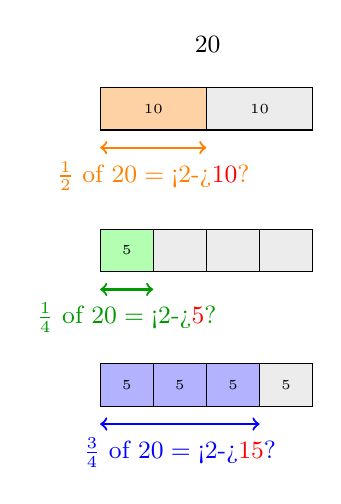
\begin{tikzpicture}[scale=0.9]
% Label for whole (20) above the top bar
\node[anchor=west] at (1.2,5.0) {\small $20$};
% Bar model for 1/2 of 20 (top)
\fill[orange!35] (0,3.8) rectangle (1.5,4.4);
\fill[gray!15] (1.5,3.8) rectangle (3,4.4);
\draw (0,3.8) rectangle (3,4.4);
\draw (1.5,3.8) -- (1.5,4.4);
\node at (0.75,4.1) {\tiny $10$};
\node at (2.25,4.1) {\tiny $10$};
\draw[<->, orange, thick] (0,3.55) -- (1.5,3.55);
\node[orange] at (0.75,3.15) {\small $\frac{1}{2}$ of $20 = \text{\ashowq{10}}$};
% Bar model for 1/4 of 20 (middle)
\fill[green!30] (0,1.8) rectangle (0.75,2.4);
\fill[gray!15] (0.75,1.8) rectangle (3,2.4);
\draw (0,1.8) rectangle (3,2.4);
\foreach \x in {0.75,1.5,2.25} \draw (\x,1.8) -- (\x,2.4);
\node at (0.375,2.1) {\tiny $5$};
\draw[<->, green!60!black, thick] (0,1.55) -- (0.75,1.55);
\node[green!60!black] at (0.375,1.15) {\small $\frac{1}{4}$ of $20 = \text{\ashowq{5}}$};
% Bar model for 3/4 of 20 (bottom)
\fill[blue!30] (0,-0.1) rectangle (2.25,0.5);
\fill[gray!15] (2.25,-0.1) rectangle (3,0.5);
\draw (0,-0.1) rectangle (3,0.5);
\foreach \x in {0.75,1.5,2.25} \draw (\x,-0.1) -- (\x,0.5);
\node at (0.375,0.2) {\tiny $5$};
\node at (1.125,0.2) {\tiny $5$};
\node at (1.875,0.2) {\tiny $5$};
\node at (2.625,0.2) {\tiny $5$};
\draw[<->, blue, thick] (0,-0.35) -- (2.25,-0.35);
\node[blue] at (1.125,-0.75) {\small $\frac{3}{4}$ of $20 = \text{\ashowq{15}}$};
\end{tikzpicture}
\end{center}

\column{0.75\textwidth}
\small
\begin{ealglossed}
\begin{enumerate}
\begin{multicols}{2}
  \item Fully \ealgloss{simplify}{uprościć}: $\dfrac{18}{24}$ \ashow{$\dfrac{3}{4}$}
  \item Calculate: $2\dfrac{1}{3} + 1\dfrac{1}{2}$ \ashow{$=3\dfrac{5}{6}$}
\end{multicols}
  \item Using the \ealgloss{bar models}{modele słupkowe} to the left:
  \[
    \tfrac{1}{2} \text{ of } 20 = \ablank{10} \qquad \tfrac{1}{4} \text{ of } 20 = \ablank{5} \qquad \tfrac{3}{4} \text{ of } 20 = \ablank{15}
  \]
  \item Calculate:
  \[
    \tfrac{1}{3} \text{ of } 24 \qquad \tfrac{2}{3} \text{ of } 24
  \]
  \ashow{$8$ and $16$}
  \item Fill in the blank: $\quad \dfrac{3}{4}$ of $\ablank{24} = 18$

\begin{multicols}{2}
  \item Find $\dfrac{2}{5}$ of $35$. \ashow{$14$}
  \vspace{2em}
  \item Amy cuts a  $60\,\text{cm}$ ribbon and takes $\dfrac{3}{4}$ of it. How long is her piece? \ashow{$45$ cm}
\end{multicols}
  \item True or false? ``$\dfrac{1}{2}$ of $30 = 30 \div 2$.'' Explain your reasoning.
  \ashow{True. $\tfrac12$ of $30 = 15$ and $30 \div 2 = 15$.}
\end{enumerate}
\end{ealglossed}
\end{columns}
\end{frame}

%------------------------------------------------
% SLIDE 16: Fractions of Amounts (Mixed difficulty)
%------------------------------------------------
\begin{frame}{Starter}

\vspace{-2em}

\begin{columns}

\column{0.22\textwidth}
\begin{center}
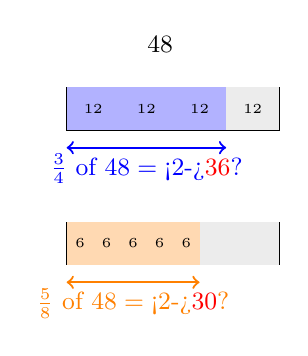
\begin{tikzpicture}[scale=0.9]

% Bar model for 3/4 of 48
\node[anchor=west] at (1, 5.5) {\small $48$};

\draw (0,4.3) rectangle (3,4.9);
\foreach \x in {0.75,1.5,2.25} \draw (\x,4.3) -- (\x,4.9);
\fill[blue!30] (0,4.3) rectangle (0.75,4.9);
\fill[blue!30] (0.75,4.3) rectangle (1.5,4.9);
\fill[blue!30] (1.5,4.3) rectangle (2.25,4.9);
\fill[gray!15] (2.25,4.3) rectangle (3,4.9);
\node at (0.375,4.6) {\tiny $12$};
\node at (1.125,4.6) {\tiny $12$};
\node at (1.875,4.6) {\tiny $12$};
\node at (2.625,4.6) {\tiny $12$};

\draw[<->, blue, thick] (0,4.05) -- (2.25,4.05);
\node[blue] at (1.125,3.75) {\small $\frac{3}{4}$ of $48 = \text{\ashowq{36}}$};

\draw (0,2.4) rectangle (3,3.0);
\foreach \x in {0.375,0.75,1.125,1.5,1.875,2.25,2.625} \draw (\x,2.4) -- (\x,3.0);
\fill[orange!30] (0,2.4) rectangle (1.875,3.0);
\fill[gray!15] (1.875,2.4) rectangle (3,3.0);
\node at (0.1875,2.7) {\tiny $6$};
\node at (0.5625,2.7) {\tiny $6$};
\node at (0.9375,2.7) {\tiny $6$};
\node at (1.3125,2.7) {\tiny $6$};
\node at (1.6875,2.7) {\tiny $6$};

\draw[<->, orange, thick] (0,2.15) -- (1.875,2.15);
\node[orange] at (0.9375,1.85) {\small $\frac{5}{8}$ of $48 = \text{\ashowq{30}}$};

\end{tikzpicture}
\end{center}

\column{0.78\textwidth}
\small
\begin{ealglossed}
\begin{enumerate}
  \item Order smallest to largest: $\dfrac{3}{8},\ \dfrac{1}{2},\ \dfrac{5}{12}$ \ashow{$\dfrac{3}{8} < \dfrac{5}{12} < \dfrac{1}{2}$}
  \item Convert $\dfrac{17}{5}$ to a \ealgloss{mixed number}{liczba mieszana}. \ashow{$3\dfrac{2}{5}$}
  \item Use the \ealgloss{bar model}{model słupkowy} to find $\dfrac{3}{4}$ of $48$ and $\dfrac{5}{8}$ of $48$. \ashow{$36$ and $30$}
  \item Calculate: $\quad \dfrac{5}{8}$ of $72$ \ashow{$=45$}
  \item $\dfrac{2}{3}$ of a class of $30$ are girls. How many boys are there? \ashow{$10$ boys}
  \item Rania says ``$\dfrac{3}{5}$ of $40 = 24$''. Is she correct? Show your working. \ashow{Yes; $\dfrac{3}{5}\times 40 = 24$.}

\begin{multicols}{2}
  \item Which is greater: \newline $\dfrac{3}{4}$ of $60$ or $\dfrac{4}{5}$ of $55$? \ashow{$\dfrac{3}{4}$ of $60$ ($=45$)}
  \item Fill in the blank:
  \[
    \frac{\ablank{5}}{8} \text{ of } 64 = 40
  \]
\end{multicols}
\end{enumerate}
\end{ealglossed}
\end{columns}
\end{frame}

%------------------------------------------------
% SLIDE 17: Multiplying Fractions (Introduction)
%------------------------------------------------
\begin{frame}{Starter}

\vspace{-2em}

\begin{columns}

\column{0.25\textwidth}
\begin{center}
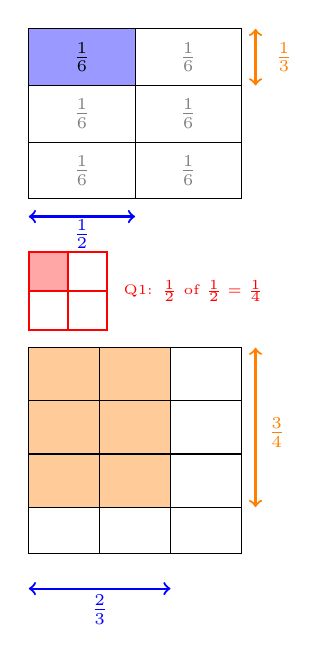
\begin{tikzpicture}[scale=0.9]

% Area model for 1/2 x 1/3

% Grid: 2 columns x 3 rows = 6 cells
\draw (0,2.5) rectangle (3,4.9);
% vertical line (halves)
\draw (1.5,2.5) -- (1.5,4.9);
% horizontal lines (thirds)
\draw (0,3.3) -- (3,3.3);
\draw (0,4.1) -- (3,4.1);

% shade 1 cell (top-left = 1/2 wide, 1/3 tall)
\fill[blue!40] (0,4.1) rectangle (1.5,4.9);

\node at (0.75,4.5) {\small $\frac{1}{6}$};
\node[gray] at (2.25,4.5) {\small $\frac{1}{6}$};
\node[gray] at (0.75,3.7) {\small $\frac{1}{6}$};
\node[gray] at (2.25,3.7) {\small $\frac{1}{6}$};
\node[gray] at (0.75,2.9) {\small $\frac{1}{6}$};
\node[gray] at (2.25,2.9) {\small $\frac{1}{6}$};

% labels on axes
\draw[<->, blue, thick] (0,2.25) -- (1.5,2.25);
\node[blue] at (0.75,2.0) {\small $\frac{1}{2}$};
\draw[<->, orange, thick] (3.2,4.1) -- (3.2,4.9);
\node[orange] at (3.6,4.5) {\small $\frac{1}{3}$};

% Area model for 2/3 x 3/4

\draw (0,-2.5) rectangle (3,0.4);
% shade 2/3 wide x 3/4 tall = 6 of 12 cells
\fill[orange!40] (0,-1.85) rectangle (2,0.4);

% vertical lines (thirds)
\draw (1,  -2.5) -- (1,  0.4);
\draw (2,  -2.5) -- (2,  0.4);
% horizontal lines (quarters)
\draw (0,-0.35) -- (3,-0.35);
\draw (0,-1.1) -- (3,-1.1);
\draw (0,-1.85) -- (3,-1.85);

% labels on axes
\draw[<->, blue, thick] (0,-3.0) -- (2,-3.0);
\node[blue] at (1,-3.3) {\small $\frac{2}{3}$};
\draw[<->, orange, thick] (3.2,0.4) -- (3.2,-1.85);
\node[orange] at (3.5,-0.8) {\small $\frac{3}{4}$};

% --- Q1 answer: 1/2 of 1/2 drawn as an area model ---
\fill[ansfill, red!35] (0,1.2) rectangle (0.55,1.75);
\draw[ans] (0,0.65) rectangle (1.1,1.75);
\draw[ans] (0.55,0.65) -- (0.55,1.75);
\draw[ans] (0,1.2) -- (1.1,1.2);
\node[anslab, right] at (1.2,1.2) {Q1: $\tfrac{1}{2}$ of $\tfrac{1}{2}=\tfrac{1}{4}$};
\end{tikzpicture}
\end{center}

\column{0.75\textwidth}
\small
\begin{ealglossed}
\begin{enumerate}
  \item What is $\dfrac{1}{2}$ of $\dfrac{1}{2}$? Draw a picture to show your answer. \ashow{$\dfrac{1}{4}$}
  \item Use the \ealgloss{area model}{model pola} on the left to calculate $\dfrac{1}{2} \times \dfrac{1}{3} = \dfrac{\ablank{1}}{\ablank{6}}$
  \item Use the second \ealgloss{area model}{model pola} to calculate and \ealgloss{simplify}{uprościć}: $\dfrac{2}{3} \times \dfrac{3}{4} = \dfrac{\ablank{6}}{\ablank{12}} = \dfrac{\ablank{1}}{\ablank{2}}$
  \item Calculate:
  \[
    \frac{3}{5} \times \frac{5}{7}
  \]
  \ashow{$=\dfrac{3}{7}$}
  \item \ealgloss{Simplify}{Uprościć} \textit{then} \ealgloss{multiply}{mnożyć}: $\quad\dfrac{3}{9} \times \dfrac{4}{8}$ \ashow{$=\dfrac{1}{6}$}
  \item Find $\dfrac{3}{4}$ of $\dfrac{2}{5}$. What do you notice about ``of'' and ``$\times$''? \ashow{$\dfrac{3}{10}$; ``of'' means multiply.}
  \item Calculate: $1\dfrac{1}{2} \times \dfrac{1}{3}$\\[0.3em]
  (Hint: convert to \ealgloss{improper}{ułamek niewłaściwy} first.) \ashow{$=\dfrac{1}{2}$}
\end{enumerate}
\end{ealglossed}
\end{columns}
\end{frame}

%------------------------------------------------
% SLIDE 18: Multiplying Fractions & Amounts (Mixed)
%------------------------------------------------
\begin{frame}{Starter}

\vspace{-2em}

\begin{columns}

\column{0.22\textwidth}
\begin{center}
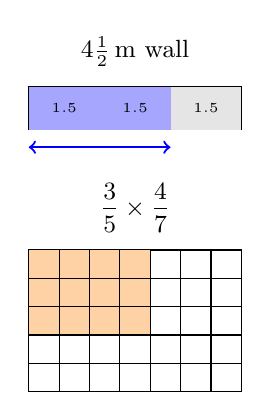
\begin{tikzpicture}[scale=0.9]

% Illustration: 2/3 of 4.5m wall
\node at (1.5, 5.3) {\small $4\tfrac{1}{2}$\,m wall};

\draw (0,4.2) rectangle (3,4.8);
\foreach \x in {1,2} \draw (\x,4.2) -- (\x,4.8);
\fill[gray!20] (0,4.2) rectangle (3,4.8);
\fill[blue!35] (0,4.2) rectangle (2,4.8);
\node at (0.5,4.5) {\tiny $1.5$};
\node at (1.5,4.5) {\tiny $1.5$};
\node at (2.5,4.5) {\tiny $1.5$};

\draw[<->, blue, thick] (0,3.95) -- (2,3.95);

% Area model reminder: 3/5 x 4/7
\node at (1.5,3.1) {\small $\dfrac{3}{5} \times \dfrac{4}{7}$};

\draw (0,0.5) rectangle (3,2.5);
\fill[orange!35] (0,1.3) rectangle (1.7143,2.5);

% 5 rows, 7 cols
\foreach \y in {0.9,1.3,1.7,2.1} \draw (0,\y) -- (3,\y);
\foreach \x in {0.4286,0.8571,1.2857,1.7143,2.1429,2.5714} \draw (\x,0.5) -- (\x,2.5);

\end{tikzpicture}
\end{center}

\column{0.78\textwidth}
\small
\begin{ealglossed}
\begin{enumerate}
\begin{multicols}{3}
  \item \ealgloss{Simplify}{Uprościć}: $\dfrac{24}{36}$ \ashow{$\dfrac{2}{3}$}
  \item $3\dfrac{1}{4} - 1\dfrac{2}{3}$ \ashow{$=1\dfrac{7}{12}$}
  \item $\dfrac{5}{6}$ of $42$ \ashow{$=35$}
\end{multicols}

  \item A wall is $4\dfrac{1}{2}$\,m long. A mural covers $\dfrac{2}{3}$ of it. Use the \ealgloss{bar model}{model słupkowy} to find the length of the mural. \ashow{$3$ m}

  \item Use the \ealgloss{area model}{model pola} to calculate: $\dfrac{3}{5} \times \dfrac{4}{7} = \dfrac{\ablank{12}}{\ablank{35}}$

  \item Which is greater: $\dfrac{2}{3} \times \dfrac{3}{4}$, or $\dfrac{3}{4}$ of $\dfrac{2}{3}$? Explain. \ashow{They are equal ($\dfrac{1}{2}$).}

\begin{multicols}{2}
  \item Fill in the blank:
  \[
    \frac{3}{5} \times \ablank{\frac{2}{7}} = \frac{6}{35}
  \]
  \newline
  \item True or false? ``\ealgloss{Multiplying}{mnożyć} two \ealgloss{proper fractions}{ułamki właściwe} always gives a smaller result than either \ealgloss{fraction}{ułamek}.'' Explain or give a \ealgloss{counterexample}{kontrprzykład}. \ashow{True; e.g.\ $\dfrac{2}{3}\times\dfrac{3}{4}=\dfrac{1}{2}$, which is smaller than both.}
\end{multicols}
\end{enumerate}
\end{ealglossed}
\end{columns}
\end{frame}

%------------------------------------------------
% SLIDE 19: Problem Solving & Mastery
%------------------------------------------------
\begin{frame}{Starter}

\vspace{-2em}

\begin{columns}

\column{0.22\textwidth}
\begin{center}
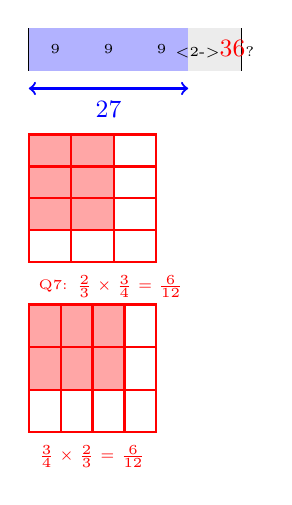
\begin{tikzpicture}[scale=0.9]

% Bar model: 3/4 of a number is 27

\draw (0,3.7) rectangle (3,4.3);
\foreach \x in {0.75,1.5,2.25} \draw (\x,3.7) -- (\x,4.3);
\fill[blue!30] (0,3.7) rectangle (2.25,4.3);
\fill[gray!15] (2.25,3.7) rectangle (3,4.3);
\node at (0.375,4.0) {\tiny $9$};
\node at (1.125,4.0) {\tiny $9$};
\node at (1.875,4.0) {\tiny $9$};
\node at (2.625,4.0) {\tiny \ashowq{36}};

\draw[<->, blue, thick] (0,3.45) -- (2.25,3.45);
\node[blue] at (1.125,3.15) {\small $27$};

% --- Q7 answer: the two area diagrams, each shading 6 of 12 cells ---
% 2/3 wide by 3/4 tall
\fill[ansfill, red!35] (0,1.45) rectangle (1.2,2.8);
\draw[ans] (0,1.0) rectangle (1.8,2.8);
\foreach \x in {0.6,1.2} \draw[ans] (\x,1.0) -- (\x,2.8);
\foreach \y in {1.45,1.9,2.35} \draw[ans] (0,\y) -- (1.8,\y);
\node[anslab, below right] at (0,0.95) {Q7: $\tfrac{2}{3}\times\tfrac{3}{4}=\tfrac{6}{12}$};
% 3/4 wide by 2/3 tall
\fill[ansfill, red!35] (0,-0.8) rectangle (1.35,0.4);
\draw[ans] (0,-1.4) rectangle (1.8,0.4);
\foreach \x in {0.45,0.9,1.35} \draw[ans] (\x,-1.4) -- (\x,0.4);
\foreach \y in {-0.8,-0.2} \draw[ans] (0,\y) -- (1.8,\y);
\node[anslab, below right] at (0,-1.45) {$\tfrac{3}{4}\times\tfrac{2}{3}=\tfrac{6}{12}$};
\end{tikzpicture}
\end{center}

\column{0.78\textwidth}
\small
\begin{ealglossed}
\begin{enumerate}
\begin{multicols}{3}
  \item \ealgloss{Simplify}{Uprościć}: $\dfrac{20}{30}$ \ashow{$\dfrac{2}{3}$}
  \item \ealgloss{Simplify}{Uprościć}: $\dfrac{84}{108}$ \ashow{$\dfrac{7}{9}$}
\end{multicols}

  \item Convert $4\dfrac{3}{5}$ to an \ealgloss{improper fraction}{ułamek niewłaściwy}. \ashow{$\dfrac{23}{5}$}

  \item Calculate: $2\dfrac{3}{4} + 1\dfrac{3}{5}$ \ashow{$=4\dfrac{7}{20}$}

  \item $\dfrac{3}{4}$ of a number is $27$. Use the \ealgloss{bar model}{model słupkowy} to find the whole number. \ashow{$36$}

  \item Jack spends $\dfrac{1}{3}$ of his pocket money on Monday and $\dfrac{1}{4}$ on Tuesday. What \ealgloss{fraction}{ułamek} remains? \ashow{$\dfrac{5}{12}$}

  \item A jug holds $1\dfrac{1}{2}$ litres. You fill $\dfrac{2}{3}$ of it. How many millilitres is that? \ashow{$1000$ mL}

  \item Show that $\dfrac{2}{3} \times \dfrac{3}{4} = \dfrac{3}{4} \times \dfrac{2}{3}$ using area diagrams.

\end{enumerate}
\end{ealglossed}
\end{columns}
\end{frame}

\end{document}